\documentclass{article}

\usepackage{graphicx}
\usepackage{tikz}
\usepackage{tikzsymbols}
\usetikzlibrary{calc,patterns,shapes.geometric}
\pagestyle{empty}
\usepackage[margin=0pt]{geometry}
\geometry{papersize={14in,12in}}

\def\centerarc[#1](#2)(#3:#4:#5){\draw[#1] ($(#2)+({#5*cos(#3)},{#5*sin(#3)})$) arc (#3:#4:#5);}

\begin{document}
	\begin{figure}
		\centering
		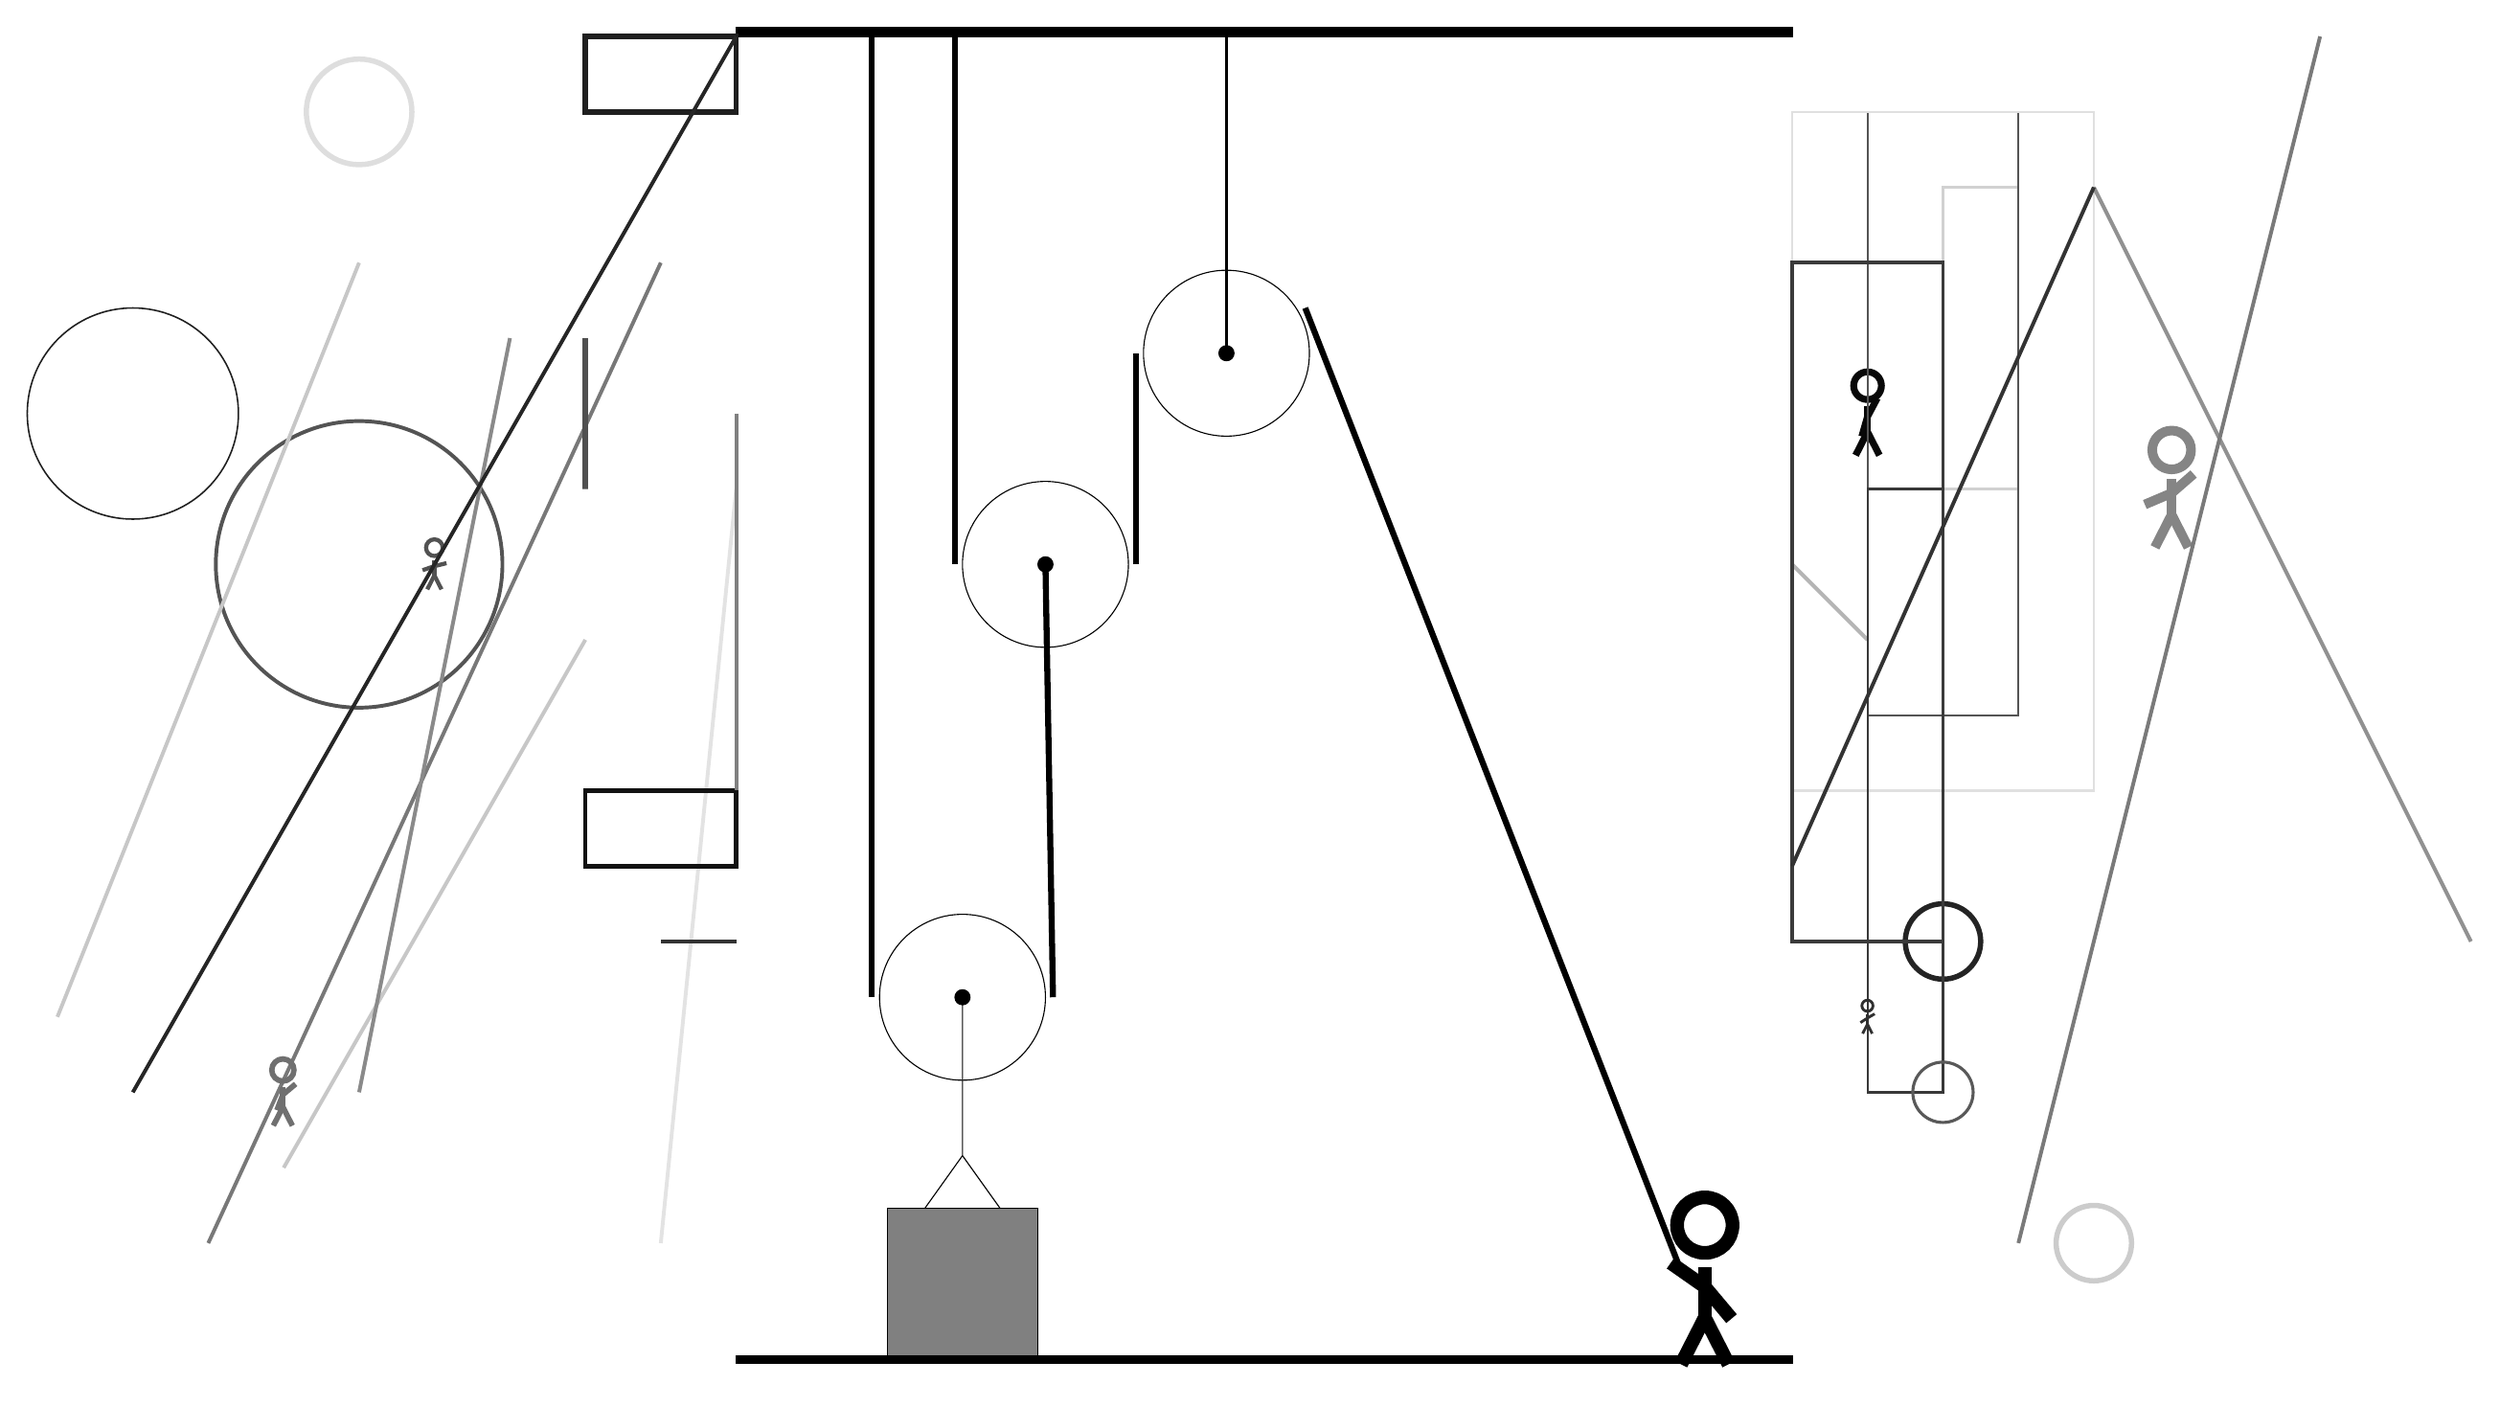
\begin{tikzpicture}
			%%%%% START %%%%%
			
			\draw[fill=black] (-2, 14) rectangle (12, 14.125);
			
			\draw (1, 1.26) circle (1.1);
			\draw[fill=black] (1, 1.26) circle (0.1);
			
			\node[line width=0.2mm, color=black!48] at (17, 8) {\Strichmaxerl[7][23][41]};
			
			\draw [line width=0.7mm, color=black!20](16, -2) circle (0.5);
			\draw[line width=0.3mm, color=black!18] (14, 12) rectangle (15, 8);
			\node[line width=0.2mm, color=black!97] at (13, 9) {\Strichmaxerl[5][74][62]};
			
			\draw[line width=0.5mm, color=black!11](-3, -2) -- (-2, 8);
			\draw[line width=0.6mm, color=black!93] (-2, 3) rectangle (-4, 4);
			
			\draw[line width=0.3mm, color=black!67] (13, 13) rectangle (15, 5);
			\draw [line width=0.5mm, color=black!67](-7, 7) circle (1.9);
			\draw[line width=0.7mm, color=black!88] (-4, 14) rectangle (-2, 13);
			\draw [line width=0.7mm, color=black!86](14, 2) circle (0.5);
			\draw[line width=0.5mm, color=black!53](-3, 11) -- (-9, -2);
			\draw [line width=0.2mm, color=black!88](-10, 9) circle (1.4);
			\draw[line width=0.3mm, color=black!12] (12, 13) rectangle (16, 4);
			\draw[line width=0.5mm, color=black!29](13, 6) -- (12, 7);
			\draw[line width=0.5mm, color=black!22](-4, 6) -- (-8, -1);
			\draw[line width=0.3mm, color=black!78] (14, 8) rectangle (13, 0);
			
			\draw [line width=0.7mm, color=black!13](-7, 13) circle (0.7);
			
			\node[line width=0.5mm, color=black!68] at (-6, 7) {\Strichmaxerl[3][19][14]};
			\draw[line width=0.5mm, color=black!50](-2, 9) -- (-2, 4);
			
			\draw[line width=0.6mm, color=black!53] (-4, 9) rectangle (-4, 9);
			\draw[line width=0.5mm, color=black!77] (14, 11) rectangle (12, 2);
			
			\node[line width=0.6mm, color=black!56] at (-8, 0) {\Strichmaxerl[4][69][40]};
			
			\draw[line width=0.5mm, color=black!43](16, 12) -- (21, 2);
			\draw[line width=0.5mm, color=black!22](-7, 11) -- (-11, 1);
			\draw[line width=0.7mm, color=black!69] (-4, 8) rectangle (-4, 10);
			\draw[line width=0.5mm, color=black!80](16, 12) -- (12, 3);
			
			\draw[line width=0.5mm, color=black!46](-7, 0) -- (-5, 10);
			\draw[line width=0.5mm, color=black!80](-2, 2) -- (-3, 2);
			\draw[line width=0.5mm, color=black!52](15, -2) -- (19, 14);
			
			\draw[line width=0.5mm, color=black!85](-2, 14) -- (-10, 0);
			\node[line width=0.2mm, color=black!81] at (13, 1) {\Strichmaxerl[2][33][30]};
			\draw [line width=0.4mm, color=black!65](14, 0) circle (0.4);
			
			\draw (2.1, 7.0) circle (1.1);
			\draw[fill=black] (2.1, 7.0) circle (0.1);
			
			\draw (4.5, 9.8) circle (1.1);
			\draw[fill=black] (4.5, 9.8) circle (0.1);
			\draw[thick] (4.5, 9.8) -- (4.5, 14);
			
			\draw (1, 1.26) -- (1, -0.84) -- (0.5, -1.54) -- (1.5, -1.54) -- (1, -0.84);
			\draw[fill=black!50] (0, -1.54) rectangle (2, -3.54);
			
			\draw[line width=0.8mm] (-0.2, 14) -- (-0.2, 1.26);
			\centerarc[line width=0.8mm](1, 1.26)(180:360:1.2000000000000002);
			\draw[line width=0.8mm](2.2, 1.26) -- (2.1, 7.0);
			\draw[line width=0.8mm] (0.9, 14) -- (0.9, 7.0);
			\centerarc[line width=0.8mm](2.1, 7.0)(180:360:1.2000000000000002);
			\draw[line width=0.8mm](3.3, 7.0) -- (3.3, 9.8);
			\centerarc[line width=0.8mm](4.5, 9.8)(30:180:1.2000000000000002);
			\draw[line width=0.8mm] (5.544, 10.4) -- (10.5, -2.3);
			
			\node at (10.8, -2.5) {\Strichmaxerl[10][-35][-50]};
			
			\draw[fill=black] (-2, -3.5) rectangle (12, -3.6);
			
			%%%%% END %%%%%
		\end{tikzpicture}
	\end{figure}	
\end{document}